\providecommand{\main}{../../..}
\documentclass[\main/dresen_thesis.tex]{subfiles}

\begin{document}
  \section{Grazing-Incidence Small-Angle X-Ray Scattering (GISAXS)}
    \label{ch:methods:gisaxs}
    In this work, grazing-incidence small-angle X-ray scattering has been performed for multiple samples at the GALAXI instrument (\refch{ch:lss:galaxi}).
    For the experiment, the sample is placed on a flat holder as shown in \reffig{fig:methods:gisaxs:samples}, that can be moved in vertical direction to center the sample and in the plane to set the beam to the center of the sample.
    Furthermore, the sample stage is tilted to set the incident angle.
    To set the desired angle, multiple scans of the beam transmission are performed, while moving the stage, to center the sample first and to be sure that the zero angle corresponds to the flat sample orientation.
    \begin{figure}[tb]
      \centering
      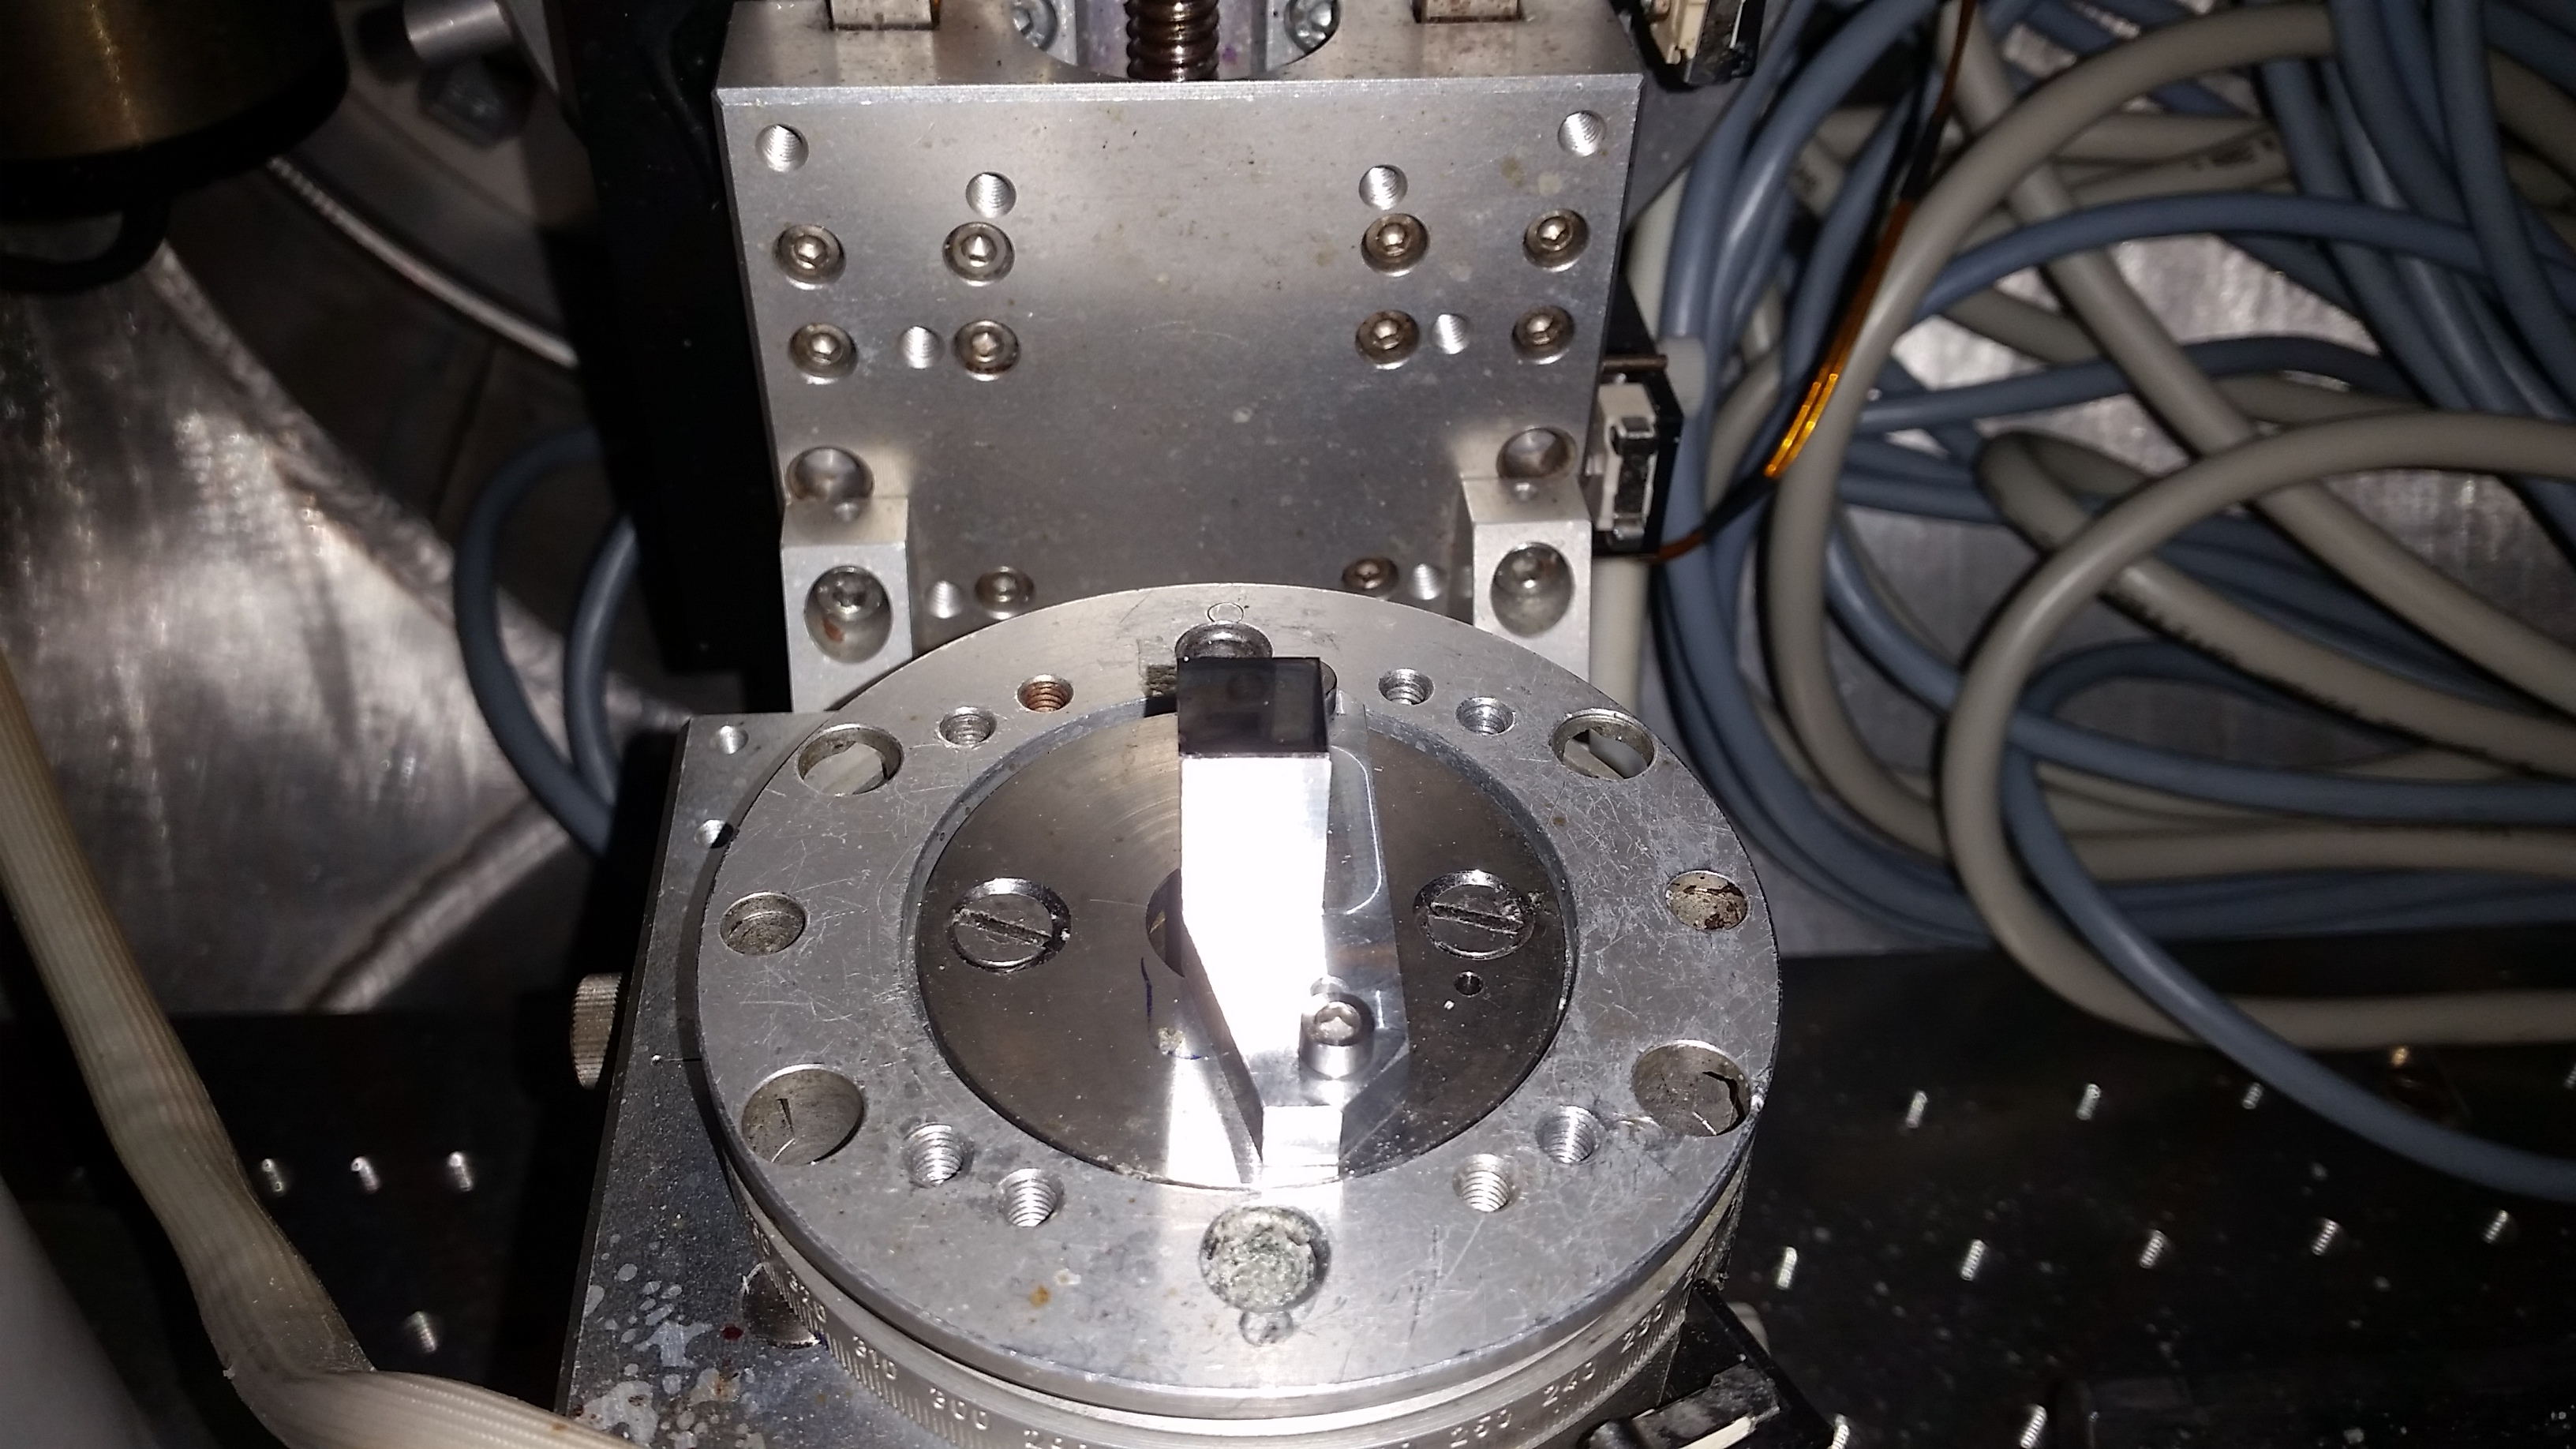
\includegraphics[width=0.7\textwidth]{appendix_methods_gisaxs_sample}
      \caption{\label{fig:methods:gisaxs:samples}For the experiment, the sample is placed on a flat surface that can be tilted and moved in all three dimensions.}
    \end{figure}

    The incident angle is set close around the critical angle of the studied material, which is typically in the order of $\alpha_\mathrm{i} \eq 0.1 \ldots 0.2 ^\circ$ at the wavelength of GALAXI for the studied materials in this thesis.
    The diffuse scattering is then integrated over a long exposure time until sufficient counting statistics are obtained.
    Typically, the samples were measured in the order of magnitude of three hours in total at one fixed incident angle.
    To remove horizontal stripes in the scattering data from the gaps between the sensitive areas of the detector, the detector is shifted multiple times vertically during the measurement in multiples of the detector pixel width.

    \begin{figure}[tb]
      \centering
      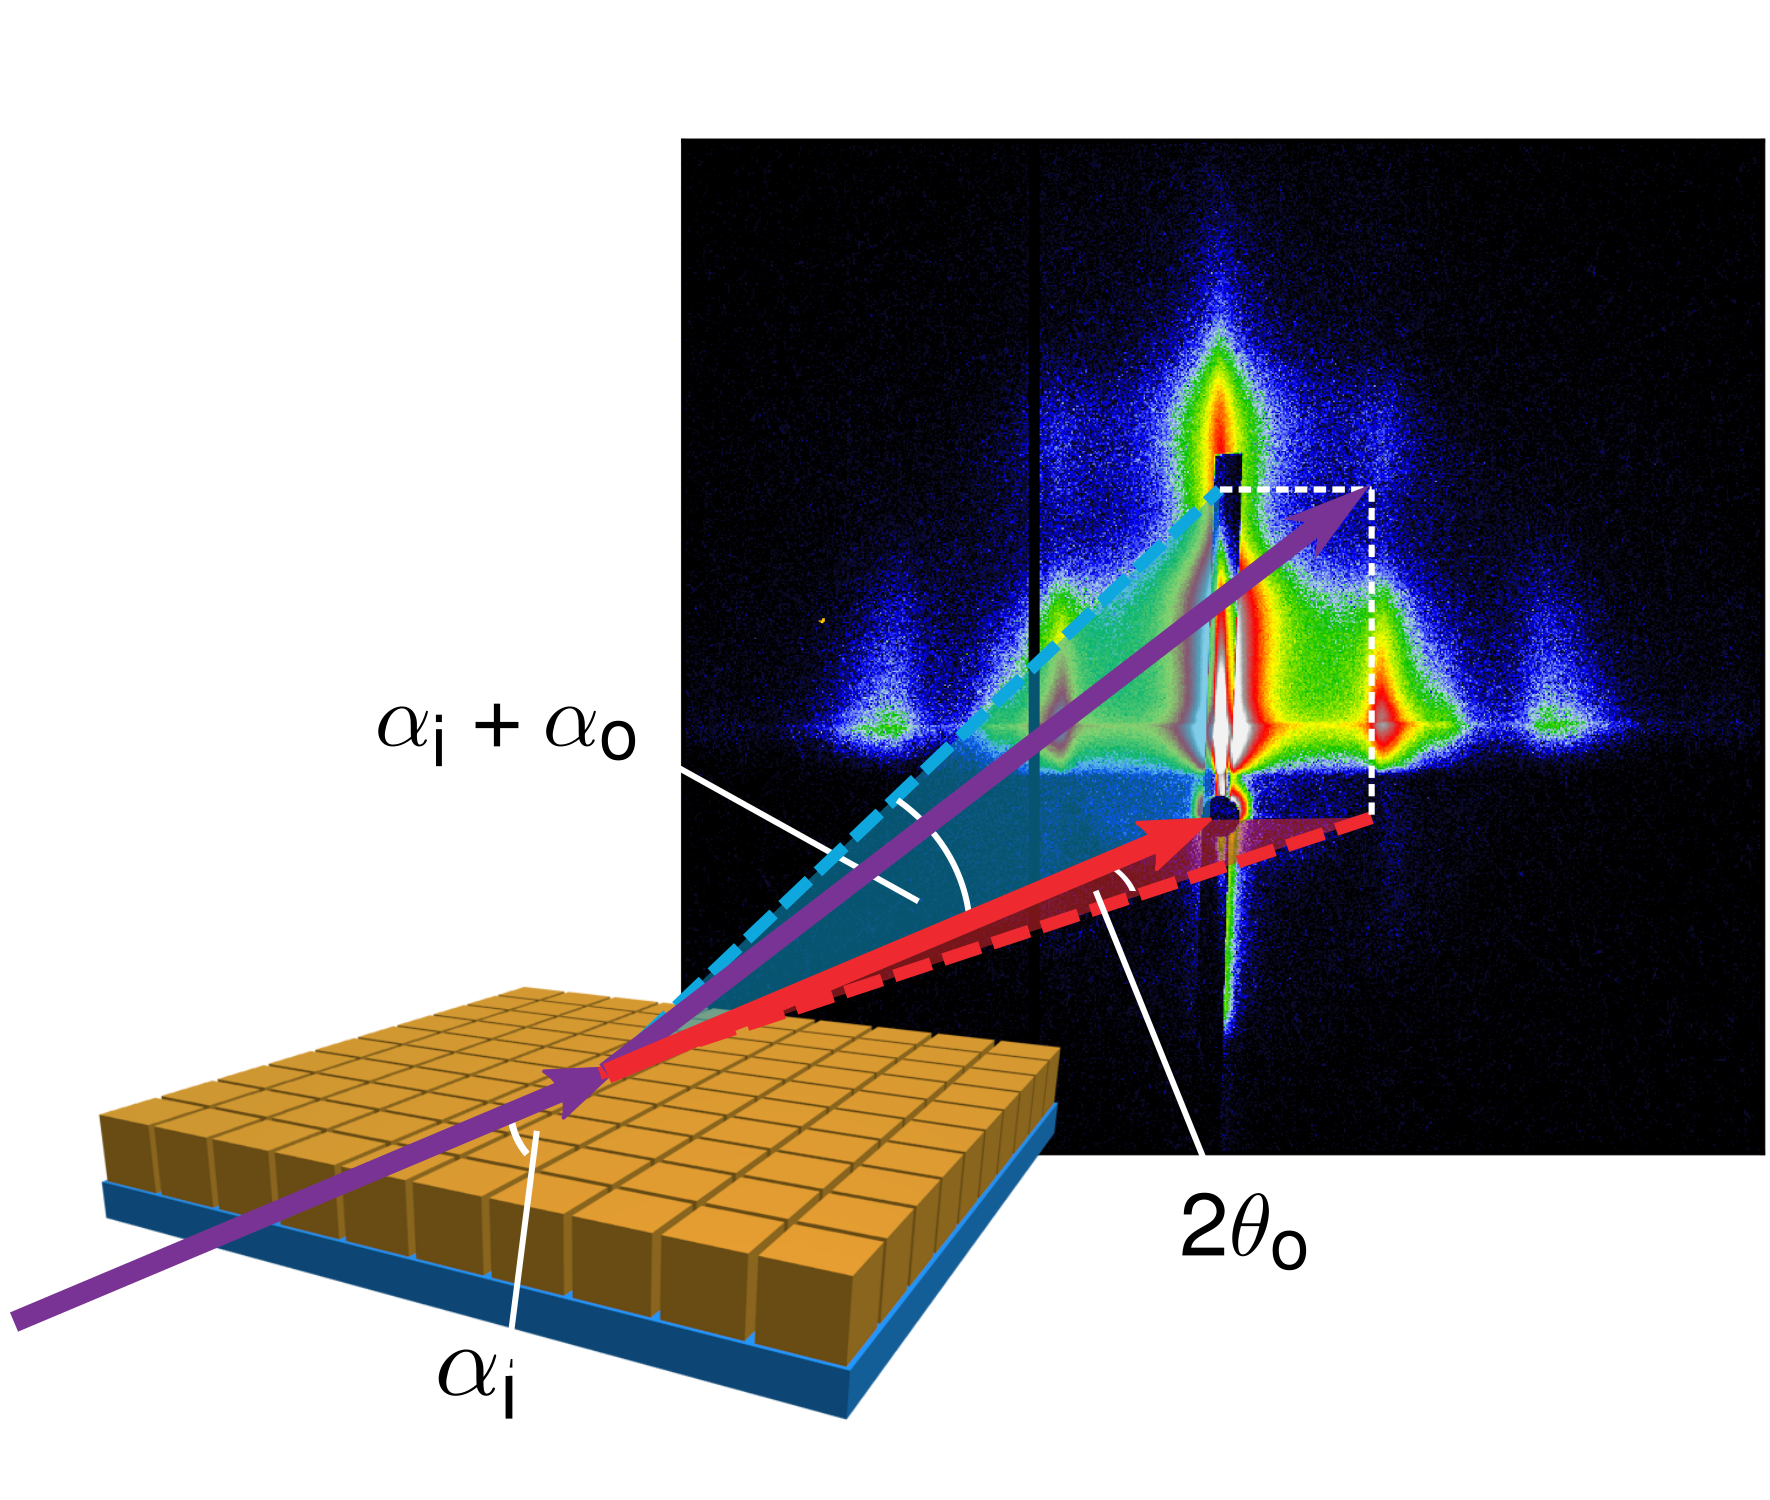
\includegraphics{appendix_methods_gisaxs_geometry}
      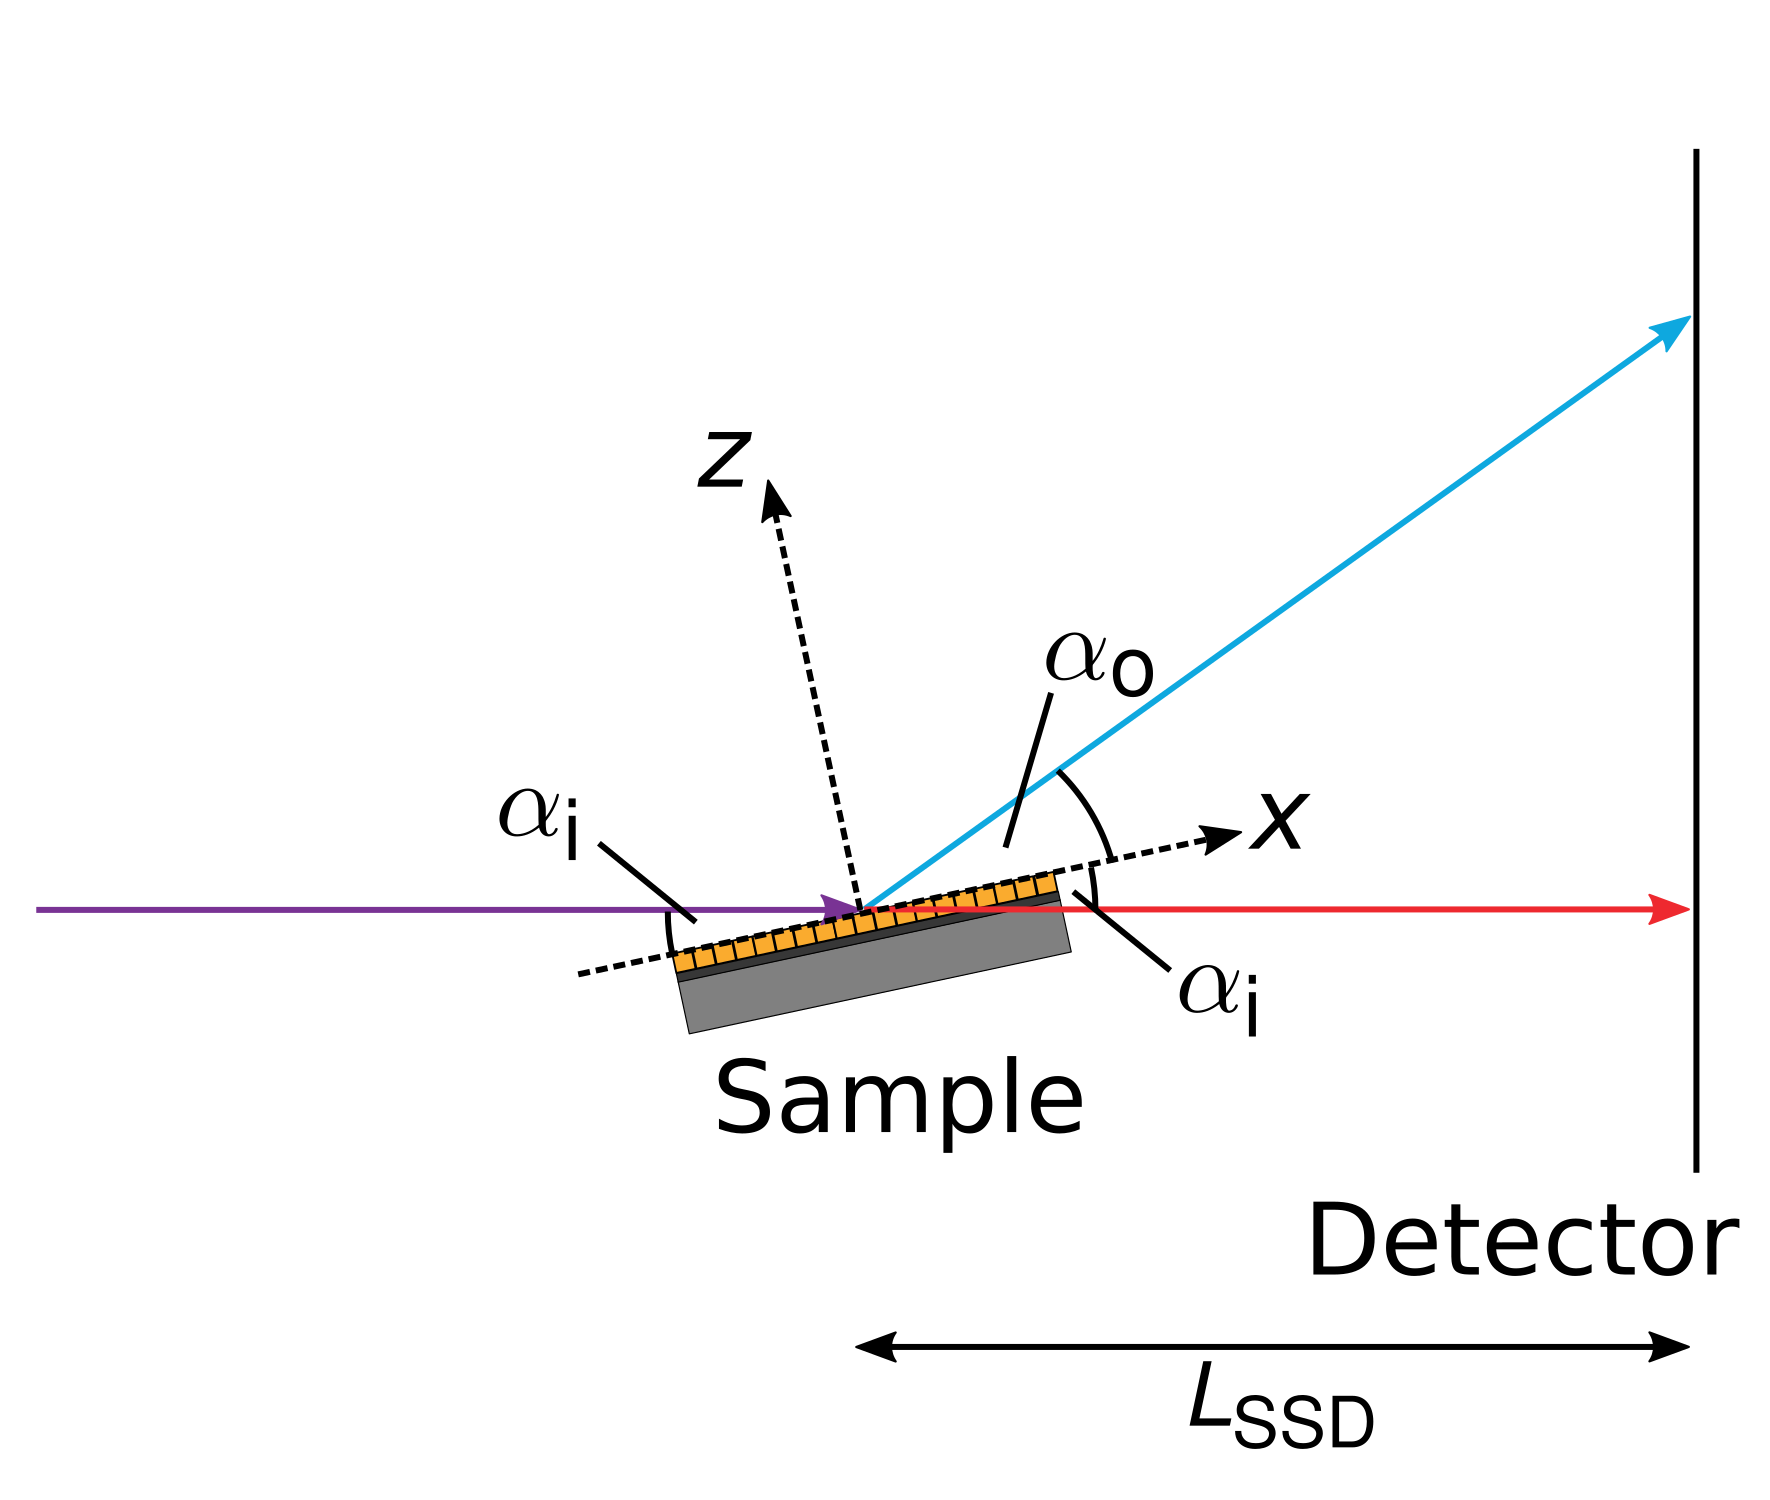
\includegraphics{appendix_methods_gisaxs_geometry2}
      \caption{\label{fig:methods:gisaxs:geometry}Geometry of a GISAXS experiments and the scattering angles: three dimensional view along the $x$-axis on the $yz$ plane (left) and a two-dimensional side view of the $xz$ plane.}
    \end{figure}

    Doing the same procedure with AgBH as described in \refapp{ch:methods:saxs}, the sample-to-detector distance $L_\mathrm{SDD}$ and the beam center position $(y_c,\,z_c)$ are determined.
    Using these, for each pixel on the detector with $(y,\,z)$ as pixel coordinate, the scattering angles are determined geometrically by comparison with \reffig{fig:methods:gisaxs:geometry}
    \begin{align}                                   
      \begin{split}
        2 \theta_\mathrm{o} &\eq \arctan \Biggl( \frac{(y - y_c) d_\mathrm{pix}}{2 L_\mathrm{SDD}} \Biggl)\\
        \alpha_i + \alpha_\mathrm{o} &\eq \arctan \Biggl( \frac{(z - z_c) d_\mathrm{pix}}{2 L_\mathrm{SDD}} \Biggl),
      \end{split}
    \end{align}
    where $d_\mathrm{pix} \eq 0.172 \unit{mm}$ is the pixel size of the detector.
    From this the incoming and outgoing wave vector, $\vec{k}_\mathrm{i}$ and $\vec{k}_\mathrm{o}$, can be read as
    \begin{align}
      \vec{k}_\mathrm{i} \eq \frac{2 \pi}{\lambda} \begin{pmatrix}
        \cos(\alpha_\mathrm{i})\\
        0\\
        -\sin(\alpha_\mathrm{i})
      \end{pmatrix}, \hspace{1cm}
      \vec{k}_\mathrm{o} \eq \frac{2 \pi}{\lambda} \begin{pmatrix}
        \cos(\alpha_\mathrm{o}) \cos(2\theta_\mathrm{o})\\
        \sin(2\theta_\mathrm{o})\\
        \sin(\alpha_\mathrm{o})
      \end{pmatrix}
    \end{align}
    and thus the scattering vector coordinates are given by
    \begin{align}
      \vec{q} \eq \frac{2 \pi}{\lambda} \begin{pmatrix}
        (\cos(\alpha_\mathrm{o}) \cos(2 \theta_\mathrm{o}) - \cos(\alpha_\mathrm{i}))\\
        \cos(\alpha_\mathrm{o}) \sin(2 \theta_\mathrm{o})\\
        (\sin(\alpha_\mathrm{i}) + \sin(\alpha_\mathrm{o}))
      \end{pmatrix}.
    \end{align}
    As only small angles are involved in GISAXS, the trigonometric functions can be linearly approximated by $\cos(x) \approx 1$ and $\sin(x) \approx x$, which yields
    \begin{align}
      \vec{q} \eq \frac{2 \pi}{\lambda} \begin{pmatrix}
        0\\
        2 \theta_\mathrm{o}\\
        \alpha_\mathrm{i} + \alpha_\mathrm{o}
      \end{pmatrix}.
    \end{align}
    or inserting the geometric parameters
    \begin{align}
      \begin{split}
        q_y &\eq \frac{2 \pi}{\lambda} \frac{(y - y_c) d_\mathrm{pix}}{L_\mathrm{SDD}}\\
        q_z &\eq \frac{2 \pi}{\lambda} \frac{(z - z_c) d_\mathrm{pix}}{L_\mathrm{SDD}},
      \end{split}
    \end{align}
    Within this coordinates, the GISAXS data is then studied with respect to characteristic length scales determined from the peak periodic length scale and peak widths.
    As well as by comparison with model calculations for the diffuse scattering calculated in the framework of the distorted-wave Born approximation.
    For this purpose, the software package BornAgain \cite{Burle_2018_borna} is helpful to formulate and calculate specific nanostructure models.
\end{document}